\documentclass[a4paper]{article}

% Load the VUB package.
% This has many options, please read the documentation at
% https://gitlab.com/rubdos/texlive-vub
\usepackage{vub}
\usepackage[english]{babel}

% Some highly suggested packages, please read their manuals.
\usepackage{hyperref}
\usepackage{float}
\usepackage{xcolor}
\usepackage{listings}
\usepackage{graphicx}
\usepackage{xparse}
\usepackage{cleveref}
\usepackage[natbib, style=ieee]{biblatex}
\usepackage{csquotes}
\usepackage{caption}
\usepackage{subcaption}
\addbibresource{bibliography.bib}
\setlength\parskip{\baselineskip}
\graphicspath{{./images}}
\definecolor{darkred}{rgb}{0.6,0.0,0.0}
\definecolor{darkgreen}{rgb}{0,0.50,0}
\definecolor{lightblue}{rgb}{0.0,0.42,0.91}
\definecolor{orange}{rgb}{0.99,0.48,0.13}
\definecolor{grass}{rgb}{0.11, 0.53, 0.17}
\definecolor{pink}{rgb}{0.97,0.15,0.45}
\definecolor{backcolour}{rgb}{0.95,0.95,0.92}

\newcommand{\secref}[1]{\autoref{#1}.}

\lstdefinestyle{mystyle}{
  basicstyle=\ttfamily,
  backgroundcolor=\color{backcolour},   
  commentstyle=\color{darkgreen}\itshape,
  keywordstyle=\color{blue}\bfseries,
  stringstyle=\color{red},
  showspaces=false,                
    showstringspaces=false,
    showtabs=false,
    breakatwhitespace=false,         
    breaklines=true,                 
    captionpos=b,                    
    keepspaces=true,                 
    numbers=left,                    
    numbersep=5pt,
}

\lstset{language=Python, style=mystyle}
\title{Delivering Actors with Stork}
\pretitle{\flushleft{Bachelor thesis submitted in partial fulfillment of the requirements for the degree of bachelor of science: Computer Science}}
\subtitle{ A distributed computing deployment tool}
\author{Gérard Lichtert}
\date{\today}
\promotors{Promotors: Prof.\ Dr.\ Joeri de Koster and Prof.\ Dr.\ Wolfgang de Meuter. \and Advisor: Mathijs Saey}
\faculty{Sciences and Bio-Engineering sciences}

\begin{document}
\maketitle
\tableofcontents
\newpage
\raggedright{}


\section{Introduction}
In a world of electronics and machines where power consumption is always increasing, optimizing power consumption is becoming increasingly important. While electricity is expensive, the main reason lies in climate change. This is because the majority of our electricity production still comes from non-renewable sources, such as coal, oil, and gas \cite{owid-energy-mix}. These sources produce a lot of CO\textsuperscript{2}, and other greenhouse gases, which are the main contributors to climate change. While there is research being done to optimize energy generation, optimizing power consumption is becoming increasingly important. This means that we as programmers can also play a role in optimizing our programs to consume less energy.

In the world of computing, cloud computing is responsible for 1\% of the worldwide energy consumption \cite{cloudcomputingenergycrisis}. To make use of the cloud, we do not only need electricity to power the devices that provide cloud computing but also electricity to power the network, which also plays a significant role in energy consumption. This is because the network is the backbone of most if not all, communication between devices and applications. The amount of connected devices and applications keeps growing, which leads to higher network usage. Consequently, higher network usage also leads to higher energy consumption, which leads to a higher carbon footprint \cite{RATHEESH}. Higher network usage also requires better infrastructure to handle the increased data volume, which in turn also requires more energy \cite{datavolumeeffects}. To reduce the network load we need to look at the data that is being sent through the network and if we can reduce it.

Data is usually transported through the network for a few reasons. Sometimes it is to send data to a device to update local data, like a chat message that needs to be added to the chat, or a new email that needs to be downloaded. While often compressed, the data is used as-is, and thus cannot be further reduced. Other times, however, data is sent to be processed. This can potentially be optimized by applying the edge-computing principle. This means that (part of) the data that is originally meant for processing is processed locally first, potentially reducing the amount of data that needs to be sent after preprocessing it. Logically, the network load, and consequently the energy consumption, should be reduced. However, for a certain set of devices or applications, it could be optimal to pre-process the complete set of data prior to sending it over the network, while for another set of devices or applications, it could be optimal to send the data directly to the server. Sometimes, however, the optimal configuration could be a combination of the two. We want to be able to experiment with these different configurations. In this work, we focus on the Python programming language, as it is a popular language often used for data science or AI applications running in the cloud. For this purpose, we introduce Stork.

Stork is a distributed computing deployment tool written in Python that makes it possible to deploy distributed systems and try out different configurations regarding these systems. More concretely, it allows us to initialize the deployment of a distributed system, change the configuration of where each part of the distributed system is deployed in a declarative way, and reverse the deployment.

In this thesis, we discuss Stork, how a user can use it and how it is implemented. We start by discussing the background of Stork. Followed by how a user can use Stork. We then discuss how Stork is implemented and finalize the thesis with a conclusion.
\section{Background}
Before we discuss Stork, we discuss the goals that Stork should achieve and how. As mentioned in the introduction, we require a tool that allows us to declare where which data gets processed. This means that we need to be able to deploy parts of our program to different devices. Consequently, this means that our tool needs to work in the context of distributed systems. For this a distributed computing paradigm is required that allows us to deploy our system in a distributed way, as well as change where parts of our programs reside. Next, we discuss the available technologies and libraries in Python and choose the one(s) that best fit our needs.
\subsection{Distributed computing paradigm}
\label{sec:distributedcomputingparadigm}
To start with distributed computing, a suitable distributed computing paradigm that allows our system to be deployed to the cloud without much manual intervention, yet helps us with experimenting different configurations, is required. There are several options, such as:
\begin{itemize}
    \item Message Passing Interface (MPI)\cite{MPI}
    \item Remote Procedure Call (RPC)\cite{RPC}
    \item Shared Memory Model\cite{SMM}
    \item The Actor Model\cite{ActorModel}
\end{itemize}
An Actor is a computational unit that encapsulates its state and behaviour, interacting with each other through asynchronous message passing. Each Actor has a mailbox in which it receives these messages and processes them sequentially. The encapsulation property of the Actor Model allows Actors to be very modular, as we can see each Actor as a separate unit that processes part of the data. More concretely, each actor will be responsible for processing a single part of the data. This allows us to easily move parts of the data processing pipeline from one device to another. This is important because we want to be able to change where data gets processed without redefining how it gets processed.

While it is technically possible to achieve modularity in MPI, RPC, and the Shared Memory Model, due to the tight coupling of those models, it is harder to achieve. This is because the state and behaviour of the system are not encapsulated in a single entity but rather spread across the entire system. This makes it harder to move parts of the system around. Consequently, we choose the Actor Model as the distributed computing paradigm for Stork.

Using an IoT system as a running example because IoT devices account for 50\% of networked devices\cite{differentnetworkneedsiot}. Say the system exists out of three devices with sensors and a cloud, where the devices feed the sensor data to the cloud. Once the data is in the cloud, it gets processed and stored in a database. It is possible to encapsulate the behaviour of each sensor in an Actor and connect this with another Actor responsible for sending the data to a server, where the data gets sent through a series of Actors that are each in turn responsible for processing a single part of the data, just like in Figure \ref{fig:iotActorExample1}.
\begin{figure}[H]
    \centering
    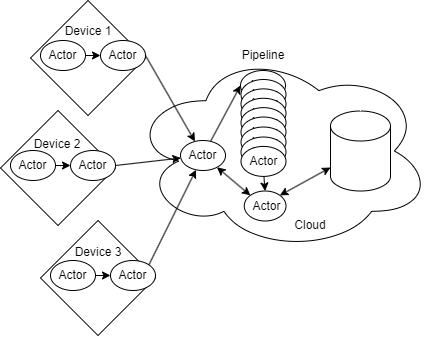
\includegraphics[width=0.6\textwidth]{iotActorExample1.png}
    \caption{An example of an IoT system using the Actor Model}
    \label{fig:iotActorExample1}
\end{figure}
Conceptually, we should be able to spawn some of the Actors that process data from the pipeline to the IoT devices and place them before the Actor that sends the data to the Server. These Actors will pre-process data prior to sending it to the cloud, where the data will go through the rest of the pipeline. The preprocessing Actors that have been moved are coloured blue and green. Achieving one of the possible configurations without having redefined how the data gets processed.
\begin{figure}[H]
    \centering
    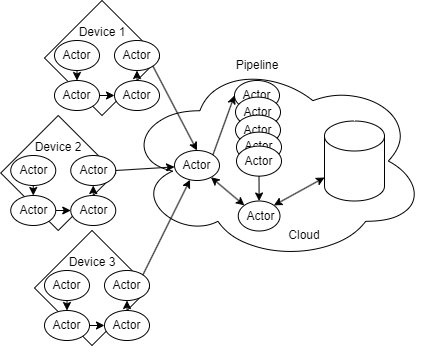
\includegraphics[width=0.6\textwidth]{iotActorsMoved.png}
    \caption{An example of an IoT system where some of the Actors that process data are spawned on the IoT devices instead of the server.}
    \label{fig:iotActorExample2}
\end{figure}
\subsection{Implementing Actors in Python}
\label{sec:implementingactors}
When using Stork to deploy distributed systems and try out different configurations, Actors have to be created. However, before we can discuss how to use Stork, we discuss how to implement Actors in Python. In Python, there are two libraries that allow us to implement the Actor Model: Pykka\footnote{https://pykka.readthedocs.io/en/stable/} and Thespian\footnote{https://thespianpy.com/doc/}. Thespian is the only library that supports distribution and distributed communication out of the box, while Pykka does not. Because of this, Thespian is the library of choice for Stork, and consequently, Stork only works with Thespian Actors.

To create an Actor, a class must inherit from a Thespian Actor class. Furthermore, this Actor must at least implement the \lstinline{receiveMessage} method or equivalent, depending on the Actor class that is extended. As mentioned in \secref{sec:distributedcomputingparadigm}, Actors communicate through asynchronous messaging. This means that when the Actor receives a message, it calls the \lstinline{receiveMessage} method. An example of an Actor implementation is given below. This Actor will respond with "Hello World! back" when it receives the message "are you there?".
\begin{lstlisting}[language=Python, caption=Actor example, label=lst:actor]
from thespian.actors import Actor

class HelloWorld(Actor):

    def receiveMessage(self, message, sender):
        if message == "are you there?":
            self.send(sender, "Hello World! back")
\end{lstlisting}
\section{Stork}
Stork is a distributed computing deployment tool, written in Python, that makes it possible to deploy an actor application over a distributed system in several different ways with minimum changes to the code. More concretely, Stork is a library that automates Actor creation on remote devices. Currently a user has to either SSH to each device to create Actors on a device, or deal with the fact that an Actor class can be initialized on a single remote device, from the cloud. Stork works around having to manually SSH to each device to create Actors and allows the user to create multiple instances of an Actor class on different remote devices by delivering the Actor class to the requested devices and creating the Actor on the device.

To illustrate the usage of Stork, we have the following example, which we will reuse throughout this section. The example consists of three remote devices and a server, which will be referred to as the leader of the distributed system. On the remote devices, data is generated. The goal of this system is to process a list of lists of integers. Out of each list of integers, the average is computed followed by the square of the average. Afterwards the data is stored on the database. As an initial configuration, where all the processing is done on the server we have the example depicted in Figure \ref{fig:config1}.
\begin{figure}[H]
    \centering
    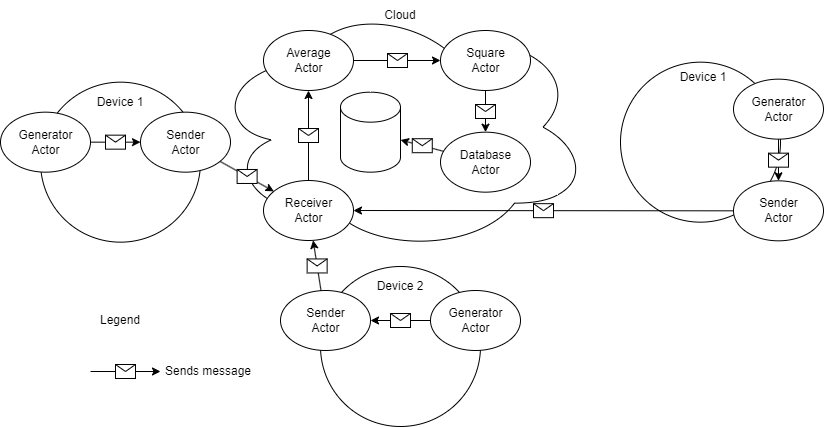
\includegraphics[width=0.8\textwidth]{systemexample1.png}
    \caption{An initial configuration where the entire pipeline is in the cloud.}
    \label{fig:config1}
\end{figure}
Here the generator Actors send a list of integers to a Sender Actor, which' sole responsibility is to forward data to the Receiver Actor in the server. The Receiver Actor forwards the received data to the processing pipeline which consists of the Average Actor and the Square Actor. Each computing the average and the square of the average respectively. The processed data is then forwarded to the Database Actor, which stores it in the database.

Another configuration is that the average is computed prior to the data being sent to the server. This means that the Average Actor would have to come before the Sender Actor on the remote devices. This configuration is depicted in Figure \ref{fig:config2}.
\begin{figure}[H]
    \centering
    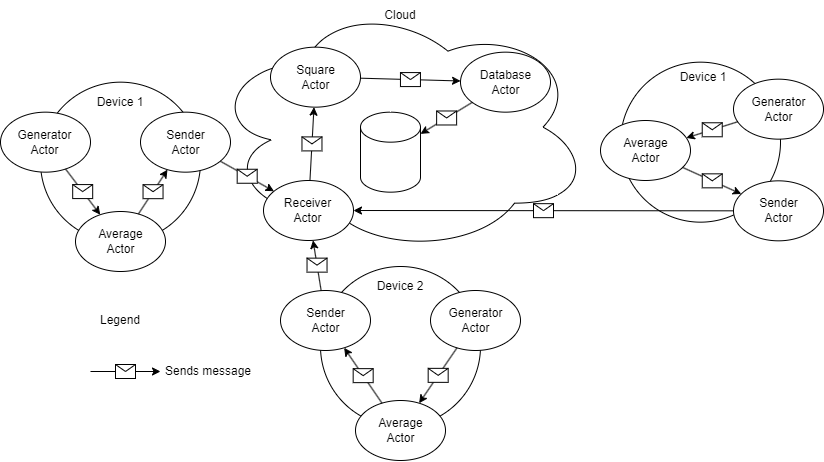
\includegraphics[width=0.8\textwidth]{systemexample2.png}
    \caption{A secondary configuration where the average is computed on the remote devices.}
    \label{fig:config2}
\end{figure}
Apart from the fact that the average is now computed prior to it being sent to the server, the configuration stays the same.

To try these different configurations, Stork stork provides the following features:
\begin{enumerate}
    \item Initializing the distributed system, allowing Actors to be spawned.
    \item De-initializing the distributed system, removing all Actors, and killing all processes related to Stork.
    \item Delivering an Actor class to devices, allowing Actors to be spawned on devices. There are two variants: \lstinline{deliverActor} and \lstinline|deliverOrActor|.
    \item Fetching the references of Actors that have been spawned across the distributed system. There are three variants: \lstinline|getActorAddress|, \lstinline|getActorClassAddresses| and \lstinline|getActorHostAddresses|.
    \item sending or broadcasting messages to the spawned Actors.
\end{enumerate}
\subsection{Initializing the distributed system}
Before creation of Actors is possible the distributed system has to be initialized. More concretely, Stork has to be present on all the devices to be able to create Actors remotely. This is because each device must have an ActorSystem running in the background to be able to create Actors. Furthermore Stork has to manage the creation and bookkeeping of Actors, and it cannot do so if the ActorSystems have not spun up before creating the Actors. To initialize the distributed system, the host names of all devices must be known and a leader of the system must be known.

Stork starts by spinning up an ActorSystem on the leader device which then connects with the rest of the system from the leader device to spin up ActorSystems on the rest of the devices. Furthermore, the bookkeeping and creation of Actors is done from the leader device. This is because the leader device is the only device that has access to the rest of the remote devices upon initialization. As an example, using the system depicted in Figure \ref{fig:config1} and Figure \ref{fig:config2}, the initialization of the distributed system is shown in Listing \ref{lst:init}.
\begin{lstlisting}[language=Python, caption=Initializing the distributed system, label=lst:init]
import Stork
devices = ["server@vub.ac.be","device1", "device2", "device3"]
Stork.distributeSystem(leader=devices[0], convention=devices)
\end{lstlisting}
When a user wants to assign certain roles to devices, Stork provides a way to do this during initialization of the distributed system. This is useful and helps the user spawn Actors on devices that have common responsibilities. More concretely, if two or more devices should have the same Actor, such as compute the average as in our example in Figure \ref{fig:config2}, the user can declare the devices in a dictionary with the keys as the host names and a list of roles that the device should have. This is shown in Listing \ref{lst:initcap}.
\vfill
\begin{lstlisting}[language=Python, caption=Initializing the distributed system with devices have common roles, label=lst:initcap]
import Stork
devices = {
    "server@vub.ac.be" : ["server", "database"],
    "device1" : ["generator", "sender"],
    "device2" : ["generator", "sender"],
    "device3" : ["generator", "sender"]
}
Stork.distributeSystem(leader=devices.keys()[0], convention=devices)
\end{lstlisting}
In Listing \ref{lst:initcap} the devices 1, 2 and 3 share the generator and sender roles, as they each have an instance of the Generator and Sender Actors in the configuration of Figure \ref{fig:config1}. Note that the host name is automatically added to the list of roles that each device has.
\subsection{De-initializing the distributed system}
Whenever a user wants to stop the distributed system, or if the user wants to change the configuration of the distributed system. For example when going from the configuration of Figure \ref{fig:config1} to the configuration of Figure \ref{fig:config2}, the distributed system must be de-initialized and re-initialized. To de-initialize the distributed system, Stork provides a method called \lstinline{undistributeSystem}. This method kills all Stork processes (including ActorSystems) on the devices. Like with the initialization method, it expects a list of the host names of the devices that are part of the distributed system and the leader of the distributed system. Again because it creates a connection from the leader device to the rest of the devices to kill the processes there first, and ends by killing the process on the leader device. Usage is shown in Listing \ref{lst:deinit}.
\begin{lstlisting}[language=Python, caption=De-initializing the distributed system, label=lst:deinit]
import Stork
devices = [ "server@vub.ac.be" ,"device1" , "device2" , "device3"]
Stork.undistributeSystem(leader=devices[0], convention=devices)
\end{lstlisting}
\subsection{Delivering an Actor class to the devices}
Now that the methods to initialize and de-initialize the distributed system have been discussed, we can discuss how to distribute the Actors. When deploying the distributed system, or more concretely, creating the Actors and connecting them, the user must be able to spawn Actors on different devices, from the cloud. Otherwise the user would have to manually create the Actors on the devices and connect them. Which, again is not scalable. For this purpose Stork provides the following two methods: \lstinline|deliverActor| and \lstinline|deliverOrActor|. However, these methods must be called within an Actor. This is because Stork uses the Actors to communicate internally, that an Actor must be spawned on a certain device. This is a limitation of Thespian, however this is further discussed in \secref{sec:creatinganddeliveringactors}. First we discuss \lstinline|deliverActor| and \lstinline|deliverOrActor|.

In Listing \ref{lst:initcap} we discussed using roles to assign common responsibilities to devices. This will be helpful when creating Actors because it uses the roles to determine on which devices the Actor should be spawned. As a limited example, using the system depicted in Figure \ref{fig:config1}, we can create the GeneratorActor using the common "generator" role. However, since we are creating these Actors from the cloud, and the method can only be called from within an Actor, we need to create another Actor that will be responsible for spawning the Generator Actors on the devices. For the following example, the responsibility of spawning the Generator Actors will be given to the GeneratorSpawner Actor.

Note that all Actors still need to implement the \lstinline{receiveMessage} method, as discussed in \secref{sec:implementingactors} even if it is empty. This is because Thespian requires it. \lstinline|deliverActor| and \lstinline|deliverOrActor| takes the actor calling the method as a first argument as well as the class of actor that must be created and a list of roles. Here is where \lstinline|deliverActor| and \lstinline|deliverOrActor| differ. \lstinline|deliverActor| checks if a device has all the roles in the list, while \lstinline|deliverOrActor| checks if the device has at least one of the roles in the list.
\begin{lstlisting}[language=Python, caption=Delivering Actors, label=lst:deliverActor]
import Stork
from thespian.actors import Actor

class GeneratorActor(Actor):

    def receiveMessage(self, message, sender):
        # generate data and send it to the sender actor

class GeneratorSpawner(Actor):

    def receiveMessage(self, message, sender):
        if message == "spawn":
            Stork.deliverActor(self, GeneratorActor, ["generator"])

\end{lstlisting}
Note that the delivery method is triggered when the spawner receives the "spawn" message. This is necessary because of another limitation of thespian, where methods making use of the asynchronous message passing cannot be called during initialization of the actor. Only after, which means that a user has to create the spawner and send "spawn" to it after it is initialized.

The example in Listing \ref{lst:deliverActor} will create Generator Actors on all devices that have the "generator" role. More concretely, there will be Generator Actors on devices 1, 2 and 3 but not the cloud. If the example used \lstinline|Stork.deliverOrActor(self, GeneratorActor, ["device1", "device2", "device3"])| instead, the result would have been the same. This is because each device has at least one of the roles in the list, and as previously mentioned, the host names are automatically added to the roles of the device.

How does a user of Stork interact with the created Actors? Whenever the delivery methods are called, Stork creates references to the created Actors and sends these references back to the actor that called the method. However, these references will be wrapped in a class called \lstinline|DeliveredActors| which not only contains the references of the created Actors but also other metadata, such as the host name of where the actor was created and the class of the actor. Since this is received as a message, the actor that called the delivery method has to handle the message in \lstinline|receiveMessage|. However, prior to showing an example, we discuss what can be done with the \lstinline|DeliveredActors| class, as it does provide some useful methods to interact with the created Actors.

Whenever a user wants to send a message to the created Actors, there are a few options of doing so. A message can be sent to a single actor, depending on its location, or more concretely host name, and class. For this the method \lstinline|emit| exists. However, if a message is meant to be sent to multiple Actors, broadcasting a message is a better solution. Depending on if a message has to be broadcasted to a specific device or to all the Actors, \lstinline|broadcast| or \lstinline|broadcastHost| can be used, respectively. If a reference to an actor needs to be saved for later use, or if the previous methods are not sufficient, it is best to unpack the class through \lstinline|unpackActors|, which returns a dictionary of the references, including the metadata. The structure is shown below in Listing \ref{lst:unpack}
\begin{enumerate}
    \item \lstinline{emit(self: Actor, host: str, Actorclass: Actor, message: Any)}: This method sends a message to the Actor that was spawned on the device with the given host name.
    \item \lstinline{broadcastHost(self: Actor, host: str, message: Any)}: This method sends a message to all the Actors that were spawned on the device with the given host name.
    \item \lstinline{broadcast(self: Actor, message: Any)}: This method sends a message to all the Actors that were spawned.
    \item \lstinline{unpackActors()}: This method returns a dictionary with the host names of the devices as keys and a list as value. The list as value contains dictionaries of the spawned Actor class as keys and the reference as value. This way we can address the Actor not only by the device that it is on but also by the class. Using the example from listing \ref{lst:deliverActor}, unpacking the class sent to the caller of the delivery method would look as follows:
          \begin{lstlisting}[language=Python, caption=lst:Unpacking structure ,label=lst:unpack]
{
"device1": [{ GeneratorActor: reference_to_GeneratorActor }],
"device2": [{ GeneratorActor: reference_to_GeneratorActor }],
"device3": [{ GeneratorActor: reference_to_GeneratorActor }]
}
    \end{lstlisting}
\end{enumerate}
As with the \lstinline|deliverActor| method, the \lstinline|DeliveredActors| class must be used within an Actor. This is because the \lstinline|DeliveredActors| class uses the Actor to send messages to other Actors. Extending the example from Listing \ref{lst:deliverActor} the next example will show a sample usage of the \lstinline|DeliveredActors| class, and broadcast to all GeneratorActors to create a SenderActor on their device. The message that triggers the creation of the Sender Actor is wrapped in a class that contains the hostname of the device where the GeneratorActor should create the SenderActor
\vfill
\begin{lstlisting}[language=Python, caption=Receiving the references of the spawned Actors and broadcasting CreateSendActor, label=lst:receive]
import Stork
from thespian.actors import Actor

class GeneratorActor(Actor):

    def receiveMessage(self, message, sender):
        if isinstance(message, CreateSenderActor):
            stork.deliverActor(self, SenderActor, [message.device])

class SenderActor(Actor):

    def receiveMessage(self, message, sender):
        # forward message to the cloud

class SpawnerActor(Actor):

    def receiveMessage(self, message, sender):
        if message == "spawn":
            Stork.deliverActor(self, ReceiverActor, ["server"])
            Stork.deliverActor(self, GeneratorActor, ["generator"])
        elif isinstance(message, Stork.DeliveredActors):
            unpacked = message.unpackActors()
            for device, v in unpacked:
                message.broadcastHost(self, device, CreateSenderActor(device))
\end{lstlisting}
Noticeably, in the example the generators are created first, then the senders. But what if the ReceiverActor from Figure \ref{fig:config1} is created before the generators and the senders are created? In this case Stork provides methods to fetch the address of an existing actor. This can be done with \lstinline|Stork.getActorAddress| which expects the Actor calling it as first argument, the host name of the device we want to get the reference of, and the class of the Actor that we want to get a reference of. Essentially the same as the \lstinline|DeliveredActors.emit| method but without the message parameter.

The second method is \lstinline|Stork.getActorClassAddresses| which works similarly to \lstinline|DeliveredActors.broadcastHost|. However instead of the hostname it expects a class. More concretely, it expects the Actor calling it as the first argument and the Actor class of which we want to get addresses as the second argument. \lstinline|Stork.getActorClassAddresses| gets all the addresses of the Actors of a specific class.

Thirdly there is \lstinline|Stork.getActorHostAddresses| which works similarly to \lstinline|DeliveredActors.broadcastHost|, but without the message parameter. It expects the Actor calling it as the first argument and the host name of the device of which we want to get the references of the Actors as the second argument. \lstinline|Stork.getActorHostAddresses| gets all the addresses of the Actors on a specific device.

Just like in \ref{lst:deliverActor} the response has to be handled in the \lstinline{receiveMessage} method. For these methods Stork provides another class, to differentiate it from the \lstinline|DeliveredActors| class. This class is called \lstinline|ActorAddresses| and has the same methods as \lstinline|DeliveredActors|.
Extending Listing \ref{lst:receive} we have the following example usage, where the ReceiverActor is created before the generators and senders. This means that the sender has to get the reference of the receiver.
\begin{lstlisting}[language=Python, caption=Fetching an actor address, label=lst:fetch]
    import Stork
    from thespian.actors import Actor
    
    class GeneratorActor(Actor):
    
        def receiveMessage(self, message, sender):
            if isinstance(message, CreateSenderActor):
                stork.deliverActor(self, SenderActor, [message.device])
            if isintance(message, DeliveredActors):
                message.broadcast("fetch receiver")
    
    class SenderActor(Actor):
    
        def receiveMessage(self, message, sender):
            if message = "fetch receiver":
                stork.getActorAddress(self, "server@vub.ac.be", ReceiverActor)
            if isinstance(message, ActorAddresses):
                receiver = message
            else: 
                # forward message to receiver

    class ReceiverActor(Actor):
        
        def receiveMessage(self, message, sender):
            # forward message to averageActor

    
    class SpawnerActor(Actor):
    
        def receiveMessage(self, message, sender):
            if message == "spawn":
                Stork.deliverActor(self, GeneratorActor, ["generator"])
            elif isinstance(message, Stork.DeliveredActors):
                if isintance(next(iter(next(iter(refs.values()))[0].keys())), GeneratorActor):
                    # checks if the DeliveredActors is a result from generating the generators
                    for device, _ in message.unpackActors():
                        message.broadcastHost(self, device, CreateSenderActor(device))
                        
    \end{lstlisting}

Till now we have worked with the examples from the initial configuration as depicted in Figure \ref{fig:config1}. However to try the configuration from Figure \ref{fig:config2} the user needs to add "average" to the list of roles of the devices 1, 2 and 3. Change the linkage by for example changing which actors create which other actors. More concretely, change the generator to create the AverageActors instead of the SenderActors, which also means that now the AverageActors need to create the SenderActors. Furthermore the receiver Actors should now forward the data to the SquareActors. After changing the linkage and the roles that each device has. It suffices to re-initialize the distributed system and spawn the actors again and the new configuration is ready to be tested.

\section{Implementing Stork}
Before discussing the implementation of Stork there are a few things that must be discussed about Thespian. When creating Actors it must be done within an ActorSystem. Meaning that on every device, on which we want to create an Actor, an ActorSystem must be present. This is because the ActorSystem manages the Actors and their communication. Consequently this means that an active ActorSystem is required on each device before we can create an Actor. This can be done by running a small script that creates an ActorSystem, nothing more, since the ActorSystem will be running in the background. This means we need to SSH to all devices and run the script on each device. For a small amount of devices this probably will not be an issue if it has to be done once or twice. However, when the distributed system is large, or the deployment is repetitive, it will be very taxing to the deployer, since it is a lot of repetitive manual work.

\subsection{Automating the deployment of ActorSystems}
To automate this, we introduce Fabric, a python library that allows us to create connections with remote devices. There is still one issue though, when using Fabric to create a connection and running a command, it expects that the process returns. It does so because it expects the command to be a foreground process. However, when creating an ActorSystem, as this starts a background process, it never returns. This is circumvented by using \enquote{tmux} before executing the program to start the ActorSystem. This ensures that the process is running in the background and the command returns. This is also how the \lstinline|Stork.distributeSystem| works, as it uses Fabric to create the ActorSystems on the devices. The \lstinline|Stork.undistributeSystem| method works in a similar way, as it uses Fabric to stop the ActorSystems on the devices. This is done by running a script that stops the ActorSystem on the devices. This script is also run in a \enquote{tmux} session, to ensure that the command returns. Essentially, both Stork methods call methods implemented for Fabric that create a SSH connection to the devices and run a command, that runs the initialization or de-initialization script. Hence the importance that this is done from the leader device.

\subsection{Creating and delivering Actors}
\label{sec:creatinganddeliveringactors}
The \lstinline|Stork.deliverActor| and \lstinline|Stork.deliverOrActor| methods work in a different manner, though they do make use of the ActorSystems that have been created by the \lstinline|Stork.distributeSystem| method. In Thespian there are two ways to create Actors. One through the ActorSystem and one through an Actor, meaning that Actors can create other Actors.
This begs the question of how we can create Actors on remote devices? More specifically from the leader device, since we do not want to have to SSH to the remote devices to create Actors there. While Thespian does support a mechanism to restrict the creation of certain Actor classes to certain devices, there is no way to guarantee that the Actor is created on multiple different devices. This is because Thespian will always create an Actor on the first ActorSystem it can. Consequently, most of the times it will spawn the Actor on the same ActorSystem.
Creating a remote Actor from the local ActorSystem is no good either, as it will either create it locally or, when using the Thespian mechanism, it will throw an error that it cannot create that Actor. This is because the mechanism only works when creating Actors from Actor, however, as mentioned before it does not work when the user wants to create an instance of an Actor on multiple devices.

To work around this, we implement an administrative Actor that has to run on the leader device. As there is only one instance of the administrative Actor, we can use Thespians restriction mechanism to our advantage. This means that we can restrict the creation of the administrative Actor to the leader device. When running the scripts to initialize the ActorSystems on all devices, the script now also creates a reference to this administrative Actor. Meaning that all remote ActorSystems are now able to communicate with an administrative Actor on the leader device. However, this still does not guarantee that the references are all pointing to the same administrative Actor. Meaning that if two remote ActorSystem ask the administrative Actor for a reference to a certain Actor, they will likely not get the same response, because they will not be asking the same Actor. This is an issue. To work around this, Thespian provides another feature called the \enquote{global Actor}, which essentially gives the Actor a name, and thus now all remote ActorSystems referencing the administrative Actor will be referencing the same Actor. To prevent users of Stork having a name clash with the administrative Actor, the name is a generated hash.

Now that we have an administrative Actor that can be referenced by all remote ActorSystems, we can use this Actor to fetch addresses as well as create Actors on the leader device. However, We cannot yet create Actors on remote ActorSystems. To achieve this, we create another administrative Actor, called a manager Actor, the manager Actor will be created on all remote ActorSystems. The only thing that the manager Actor does is, register itself with the administrative Actor, create Actors on the device it resides in, followed by returning the reference of the Actors it created to an aggregator Actor. The aggregator Actor is created by the administrative Actor to collect the references of the created Actors, as per the aggregator pattern \cite{aggregatorpattern}. The manager Actor registers itself to the administrative Actor by sending its reference to the administrative Actor, as well as the hostname of the device it resides in. This way the administrative Actor can ask the manager Actor to create an Actor on the device it resides in. The manager Actor then creates the Actor and forwards the reference to the aggregator Actor. When all the references are collected by the aggregator Actor, it sends the result back to the administrative Actor as well as to the Actor that requested the creation of the Actors. This way other Actors can ask the administrative Actor for the addresses of the Actors that were created on the remote devices, and the Actor that originally requested the creation of the Actors has the reference of the Actors that were created on the remote devices. To illustrate this we have the following Actors: Ping and Pong, where the Ping Actor spawns a Pong Actor and sends it "ping", to which the pong actor replies with "pong".

When a user wants to create a Pong actor on the device with the capability \enquote{sensor} from the Ping Actor which is on a remote device. The Ping Actor sends a request to the administrative Actor on the leader device to create a Pong Actor on all the devices with the \enquote{sensor} capability.
\begin{figure}[H]
    \centering
    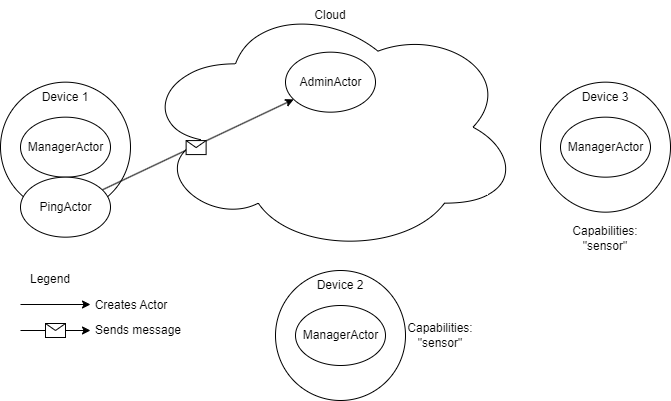
\includegraphics[scale=0.5]{createActor1.png}
    \caption{Ping sends a request to spawn Pong Actors on all devices with the \enquote{sensor} capability}
    \label{fig:createActor1}
\end{figure}
When the administrative Actor processes this request, it collects the references of the registered manager Actors that that are on remote devices with the requested capability. It counts the amount of manager Actors that it should create the Pong Actor and creates an aggregator Actor. The administrative Actor sends to the aggregator Actor the reference of the Ping Actor, that requested the creation of the Pong Actors, as well as the expected amount of results. Furthermore the administrative Actor forwards the creation request to the Manager Actors with the reference of the Aggregator Actor.
\begin{figure}[H]
    \centering
    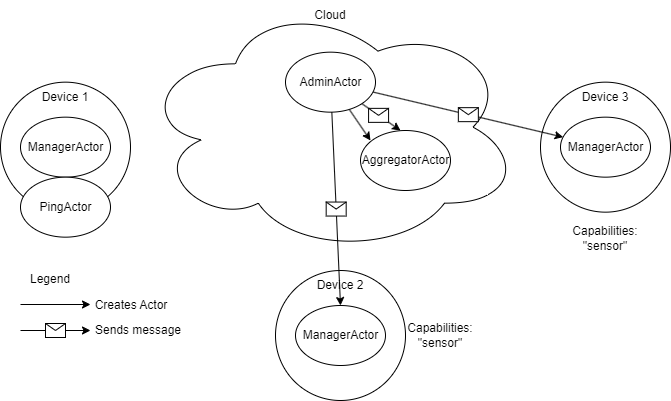
\includegraphics[scale=0.5]{createActor2.png}
    \caption{The creation request is forwarded and an aggregator Actor is created to collect the references of the created Actors}
    \label{fig:createActor2}
\end{figure}
Upon receiving the creation request from the administrative Actor, the Manager Actor creates the Pong Actor and sends the reference of the Pong Actor to the aggregator Actor.
\begin{figure}[H]
    \centering
    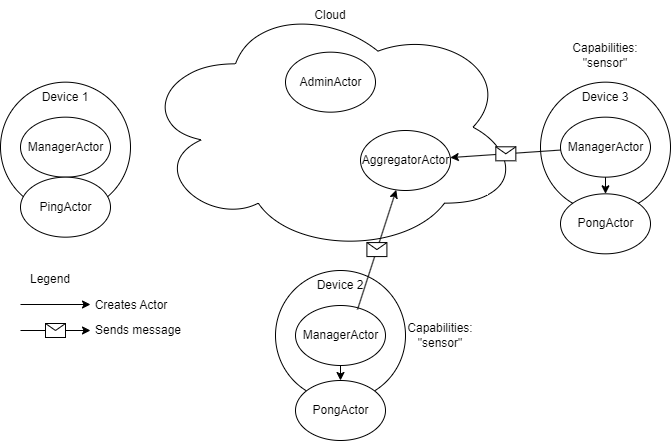
\includegraphics[scale=0.5]{createActor3.png}
    \caption{The Manager Actor creates the Pong Actor and sends the reference to the aggregator Actor}
    \label{fig:createActor3}
\end{figure}
When the aggregator collected all the expected results, it sends the collected references to both the Ping Actor as well as the administrative Actor. The administrative Actor will update its collection of Actor references while the Ping actor will only get the created references.
\begin{figure}[H]
    \centering
    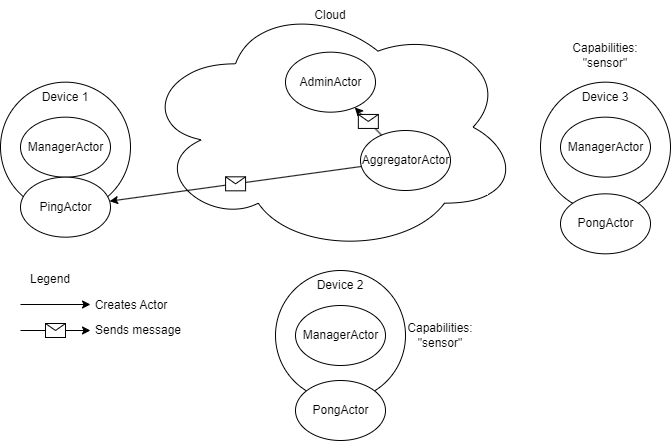
\includegraphics[scale=0.5]{createActor4.png}
    \caption{The aggregator Actor sends the collected references to the Ping Actor and the administrative Actor}
    \label{fig:createActor4}
\end{figure}
This concludes the creation of the Pong Actors on the remote devices, however in the example from listing \ref{lst:receive} the Ping Actor also sends a message to the Pong Actors. While this can be done with looping over the references and sending the message, it helps to have a method that can send a message to all the created Actors, or a subset of the created Actors. For this purpose the methods from the \lstinline|DeliveredActors| are implemented. Schematically it goes as follows:
\begin{figure}[H]
    \centering
    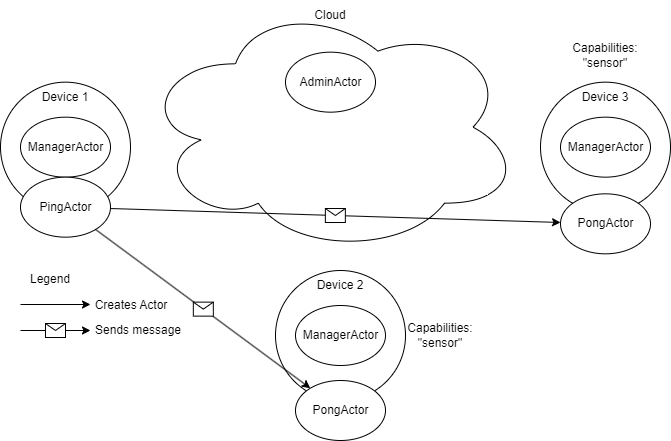
\includegraphics[scale=0.5]{createActor5.png}
    \caption{Ping broadcasts "ping" to all the created Pong Actors}
    \label{fig:createActor5}
\end{figure}
\begin{figure}[H]
    \centering
    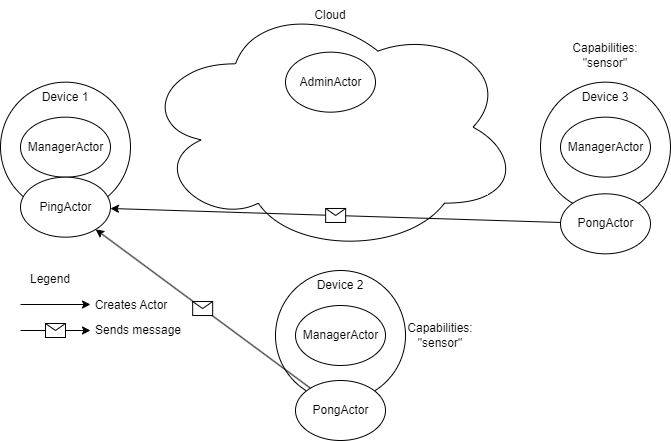
\includegraphics[scale=0.5]{createActor6.png}
    \caption{The Pong Actors receive the message and send "pong" back to the Ping Actor}
    \label{fig:createActor6}
\end{figure}
\subsection{Getting Actor references}
The \lstinline|Stork.getActorAddress|, \lstinline|Stork.getActorClassAddresses| and \lstinline|Stork.getActorHostAddresses| methods work in a similar manner. However the requests do not go further than the administrative Actor, as depicted in figure \ref{fig:createActor1}. The administrative Actor will collect the results from its collection and return the results to the Actor that requested the references. Like with the \lstinline{DeliveredActors} class, it could prove to be useful if we can interact with the Actors directly, instead of the user having to implement a method themselves. This is why the \lstinline{ActorAddresses} class has the same methods as the \lstinline{DeliveredActors} class.
\section{Conclusion}
At the beginning of this bachelor thesis, we wanted to be able to try out different configurations of distributed systems, without much manual intervention. We wanted to do this to see which configuration was the most energy efficient. To achieve this, we introduced Stork, a distributed computing deployment tool, written in Python that makes it possible to deploy distributed systems and removes the overhead of having to SSH to each device to initialize the distributed system manually. It also provides features to create Actors on remote devices, which is necessary to try out a configuration of the distributed system. To test out another configuration of the distributed system, or more concretely moving Actors around. It suffices for the user to change the flow of data, call the \lstinline|Stork.undistributeSystem| method, change the configuration of the capabilities that each device has, and call \lstinline|Stork.distributeSystem| again, before creating the Actors.

Essentially it boils down to changing the flow of data and changing some strings in a dictionary. This is a lot less work than having to SSH to each device manually, start an ActorSystem on each device and then return to the leader device. Especially when the user will still be required to create the Actors on the leader device, SSH to the remote devices again to create the Actors there and then return to the leader device to try out a single configuration. Depending on the amount of devices, configurations and the amount of times the user wants to try out a configuration, this can be very time consuming and not to mention energy inefficient, especially when a tool like Stork exists.
\printbibliography
\end{document}